\documentclass[12pt]{article}
\usepackage{amsthm,amssymb,amsfonts,amsmath,amstext,systeme}
\usepackage{graphicx,float}
\marginparwidth 0pt
\oddsidemargin -1.2 truecm
\evensidemargin  0pt 
\marginparsep 0pt
\topmargin -2.2truecm
\linespread{1}
\textheight 25.8 truecm
\textwidth 18.5 truecm
\newenvironment{remark}{\noindent{\bf Remark }}{\vspace{0mm}}
\newenvironment{remarks}{\noindent{\bf Remarks }}{\vspace{0mm}}
\newenvironment{question}{\noindent{\bf Question }}{\vspace{0mm}}
\newenvironment{questions}{\noindent{\bf Questions }}{\vspace{0mm}}
\newenvironment{note}{\noindent{\bf Note }}{\vspace{0mm}}
\newenvironment{summary}{\noindent{\bf Summary }}{\vspace{0mm}}
\newenvironment{back}{\noindent{\bf Background}}{\vspace{0mm}}
\newenvironment{conclude}{\noindent{\bf Conclusion}}{\vspace{0mm}}
\newenvironment{concludes}{\noindent{\bf Conclusions}}{\vspace{0mm}}
\newenvironment{dill}{\noindent{\bf Description of Dill's model}}{\vspace{0mm}}
\newenvironment{maths}{\noindent{\bf Mathematics needed}}{\vspace{0mm}}
\newenvironment{inst}{\noindent{\bf Instructions}}{\vspace{0mm}}
\newenvironment{notes}{\noindent{\bf Notes }}{\vspace{0mm}}
\newenvironment{theorem}{\noindent{\bf Theorem }}{\vspace{0mm}}
\newenvironment{example}{\noindent{\bf Example }}{\vspace{0mm}}
\newenvironment{examples}{\noindent{\bf Examples }}{\vspace{0mm}}
\newenvironment{topics}{\noindent{\bf Topics}}{\vspace{0mm}}
\newenvironment{outcomes}{\noindent{\bf Expected Learning Outcomes}}{\vspace{0mm}}
\newenvironment{lemma}{\noindent{\bf Lemma }}{\vspace{0mm}}
\newenvironment{solution}{\noindent{\it Solution}}{\vspace{2mm}}
\newcommand{\ds}{\displaystyle}
\newcommand{\un}{\underline}
\newcommand{\bs}{\boldsymbol}

\begin{document}
\baselineskip 18 pt
\begin{center}
{\bf \LARGE Proposal Report on IRIS}
\end{center}
\vspace{0.3cm}
\section*{Introduction}
Many people today suffer from severe psychological issues. About one in seven Hong Kong residents suffer from a mental illness or problem [1]. Patients who require assistance have to go to the clinic on their own. This is a fundamental issue; patience might not look for assistance on its own. If assistance is not sought, the issue will get worse. Hence, we developed an app to assist them in tracking their mental condition in order to improve the quality of their mental health and potentially provide some professional assistance. The proposal that follows will give a literature evaluation of recent goods. Then we'll describe our product's characteristics and operation. Finally, we'll talk about its viability and advantages.


\section*{Literature Review}
\subsection*{Smartwatch}
Smartwatch is one of the famous electronic devices nowadays. Users may keep track of their heart rate by tracking data from smartwatch sensors. Optical heart rate sensors, sometimes referred to as photoplethysmography sensors, are frequently used in smartwatches like the Fitbit Charge and Apple Watch [2-3]. The sensor may instantly transmit the user's heart rate to a device linked to the smartwatch. But with so many different smartwatch models available from tech companies, it's challenging to develop a special method for monitoring a user's mental condition and always offering a matching remedy. As a result, these smartwatches can be used to monitor a user's health, but it is challenging to offer solutions based on the health condition.


\subsection*{Do Not Disturb Mode}
Apple recently developed the Do Not Disturb system. Users are able to suppress calls and prevent notifications [4]. In order to prevent users from being distracted by pop-up notifications when they need to concentrate on work, there is a default "Do Not Disturb" mode that will block calls and notifications that may appear on the home page. Additionally, users can alter several modes and decide which phone numbers to block or allow to appear. Do Not Disturb mode is one of the finest options for people who find it difficult to concentrate while working because most people are often distracted by their phones.
\newpage

\section*{Design Description}
\subsection*{Overview and purpose}
We want to start with the most common gadget everyone owns, a smartphone, to improve mental wellness. IRIS, or Intelligent Reinforced Inner Support, is the name of our product. IRIS is software that can sync with a smartwatch, monitor a user's mental health, and offer suggestions for improvement. Our app's objective is to offer proactive assistance to raise people's quality of life.


\subsection*{Components Description}
\begin{figure}[H]
    \centering
    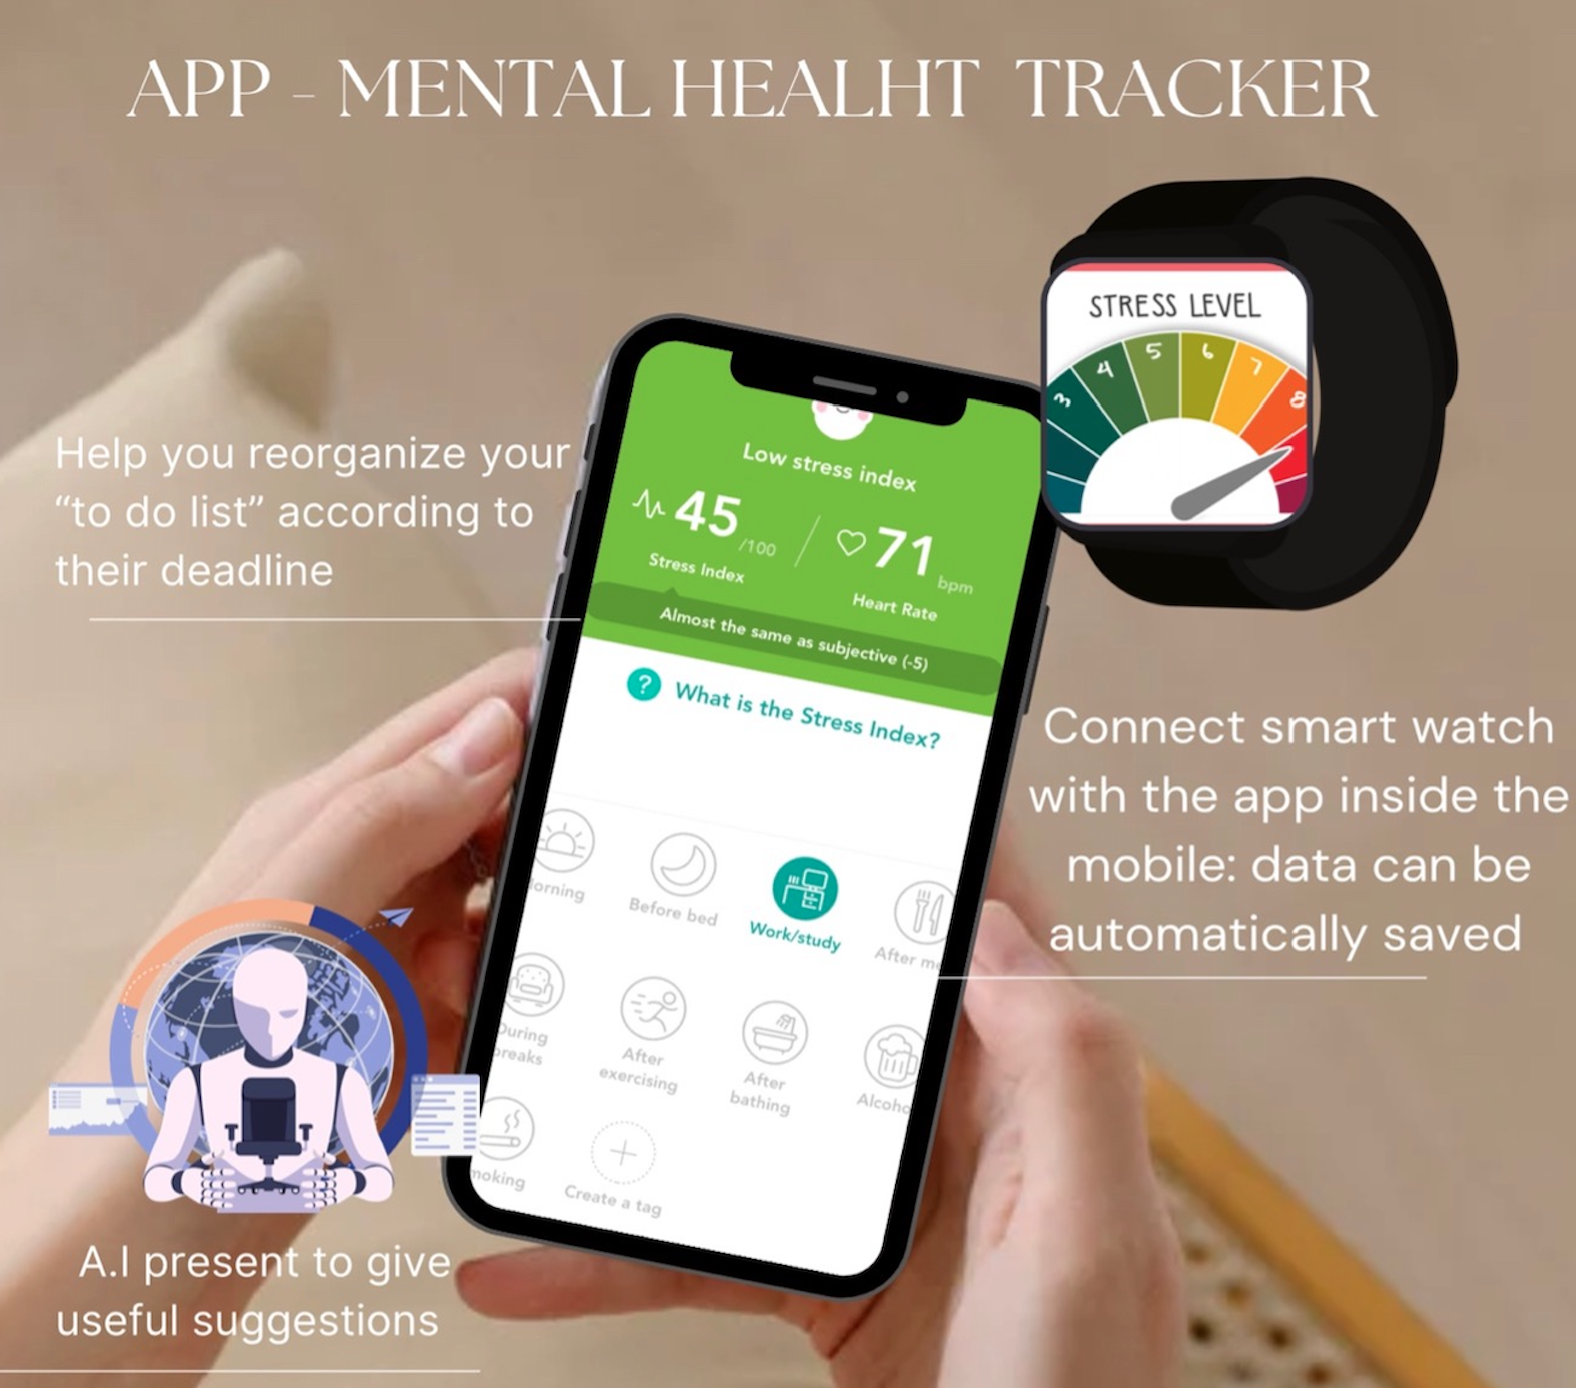
\includegraphics[width = .5\linewidth]{Figure1}
\end{figure}


According to the figure, IRIS integrates a smartwatch, an AI chatbot, and a user interface, as seen in the picture. Smartwatches are used to gather information so that we can understand the user's psychological condition better. Additionally, we offer a qualified AI chatbot for therapeutic purposes. To enhance the effectiveness of therapy chatbots, we will ask licensed psychologists and therapists to evaluate conversations between AI and users.


\subsection*{Design Operation}
The user's biometric data, including heart rate and sweat, will be first collected by the app from sensors in the smartwatch. The software then assesses the user's mental state and employs several tactics in accordance with the circumstances. For instance, non-urgent notifications will be disabled in order to give the user a peaceful environment and enhance his mental state. We also have a therapeutic chatbot, but if the problem is significant, the chatbot advises users to get professional care. This is because they could be reluctant to ask for assistance or speak to a real person.


\section*{Feasibility and Benefits Analysis}
\subsection*{Instant Assistance}
First and foremost, users have access to immediate assistance as needed. The software will gather the user's biometric data before analyzing their psychological state to check if they are experiencing any psychological issues. For instance, the software will block nearly all alerts and give users breathing exercises to help them feel better if they are having a panic attack and may not know what to do at the moment. A therapist or psychiatrist may give you medication, but none of them can provide us with the immediate help we need when we need it. Therefore, it is crucial to have mental health tracking software that can offer the right assistance when we need it.

\subsection*{Enhancing Productivity}
Secondly, with IRIS, user productivity can be raised. Controlling notifications is one of IRIS's key responsibilities. For users, this may offer a variety of relevant settings. Many people find it difficult to focus when working due to pop-up notifications on their phones, which divert their attention from the task at hand. With the help of the algorithm included in IRIS, communications can be categorized and filtered according to their value to the user. IRIS has the ability to filter out messages that are irrelevant, such as junk mail and messages from friends, when the user needs a concentrated environment to work in. A good working environment can increase user productivity without the distraction of eye-catching pop-up notifications.


\subsection*{A Good Friend}
Last but not least, IRIS can give users someone to talk to, so they can let off steam. We all need a method to communicate our emotions, therefore talking might help us release stress and feel better, claims BetterHealth [5]. To be honest with people about our concerns, though, can be difficult at times. Users can communicate with the AI therapy chatbot in IRIS to perform therapeutic sessions. They may be able to express themselves through this without having to do it in front of others. We believe that by communicating with people and expressing oneself, IRIS can help users decompress and relieve tension.







\section*{Conclusion}
In conclusion, not only can our products offer professional treatments, but they may also assist in lowering the user's stress level. IRIS may assess mental state using sensors on the smartwatch and provide appropriate suggestions, such as filtering non-urgent messages or other useful suggestions. Additionally, when users want a focused atmosphere, irrelevant messages are blocked out. Users of this cutting-edge tool can work more efficiently, feel less stressed, and have more time to do anything they want.



(1011 words)

\end{document}

